\newpage

\section{Pomoci Fourierova obrazu funkce $f(t)$ urcete Fourieruv obraz funkce $g(t)=f(3t-2)$}

Toto je novy tip prikladu. Je to hrani si se vzorci na ruzne posuny apod. Narozdil od predchozich prikladu nevime, jak vypada funkce $f(t)$ a ani nas to nezajima. Definujeme pouze, ze jeji Fourieruv obraz je $\hat{f}(p)$ a chceme vyjadrit Fourieruv obraz funkce $g(t)$, tedy $\hat{g}(p)$ v zavislosti na $\hat{f}(p)$. 

V prvnim kroku si funkci $g(t)$ upravime, potrebujeme ziskat promenou $t$ s nasobnosti 1, vzorce pro $nt$ nemame, tedy:

$$g(t) = f(3\left(t-\frac{2}{3}\right))$$

Clen $\left(t-\frac{2}{3}\right)$ nas vede na vzorec posun ve vzoru (\ref{eq:p_vzoru}). Clen $3\cdot()$ na vzorec zmeny meritka (\ref{eq:zm_meritka}). Musime dat pozor, v jakem poradi vzorce uplatnujeme. Zamena by nam ovlivnila vysledek. Postupuje z vnejsku, tedy prvni prijde naradu zmena meritka, mohla bych to napsat vse najednou, ale pro prehlednost a korektnost si zavedu funkci 
$$g_1(t)=f(3t)$$
A jeji Fourierova transformace je:
$$\hat{g_1}(p) = \frac{1}{|3|} \hat{f}\left( \frac{p}{3}\right) =  \frac{1}{3} \hat{f}\left( \frac{p}{3}\right)$$
Funkce $g(t)$ je pak:
$$g(t) = g_1 \left( t-\frac{2}{3} \right)$$ 
a jeji Fourierova transformace:
$$\hat{g}(p) = \frac{1}{3} \hat{f}\left( \frac{p}{3}\right)\cdot e^{-jp\frac{2}{3}}$$
Pro uplnost, kdybychom to chteli napsat vse naraz, tak by to bylo:
$$\hat{g}(p) = \frac{1}{|3|} \cdot F\{ f\left(t-\frac{2}{3}\right) \} \left( \frac{p}{3}\right) = \frac{1}{3} \hat{f}\left( \frac{p}{3}\right)\cdot e^{-jp\frac{2}{3}}$$

\newpage
\section{Pomoci Fourierove obrazu funkce $f(t)$ urcete Fourieruv obraz funkce $g(t)=tf(2t+1)$}

Funkce $g_1(t)=f(2t+1)$ je to same, co jsme resili v predchozim prikladu. $t$ navic nas navadi na pouziti vzorce derivace obrazu (\ref{eq:der_obr}). Meli bychom pro korektnost jeste rici, ze Fourieruv obraz funkce $f(t)$ je $\hat{f}(p)$, neboli:
$$F\{ f(t) \} = \hat{f}(p),$$
aby meli matematici radost. Mozna by za to strhli nejaky pulbodik a to nechceme. Dale urcime Fourierovu transformace funkce $g_1(t)= f(2\left(t+\frac{1}{2}\right))$:

$$\hat{g_1}(p) = \frac{1}{|2|} \cdot F\{ f\left(t+\frac{1}{2}\right) \} \left( \frac{p}{2}\right) = \frac{1}{2} \hat{f}\left( \frac{p}{2}\right)\cdot e^{jp\frac{1}{2}}$$
A pouzijeme vzorec (\ref{eq:der_obr}):
$$g(t) = t\cdot g_1(t)$$
$$\hat{g}(p) = j\frac{d}{dp}\hat{g_1}(p) = j \left( \frac{1}{2} \hat{f}\left( \frac{p}{2}\right)\cdot e^{jp\frac{1}{2}}\right)'$$
Konstantu $\frac{1}{2}$ muzeme vytknout pred derivovani a jinak se jedna o derivovani soucinu dvou funkci. Nesmime zapomenout, ze funkci $\hat{f}\left( \frac{p}{2} \right)$ musime derivovat jako slozenou funkci, tedy:
$$\frac{d}{dp}\hat{f}\left( \frac{p}{2} \right) = \hat{f}'\left(\frac{p}{2}\right) \cdot \frac{1}{2},$$
kdy prave $\frac{1}{2}$ nakonci vyrazu je vysledkem derivace vnitrni funkce.
Stejne tak funkce $e^{jp\frac{1}{2}}$ je slozena, jeji derivace je:
$$\frac{d}{dp}e^{jp\frac{1}{2}} = e^{jp\frac{1}{2}} \cdot \frac{j}{2}$$
Kdyz to spojime tedy dohromady dle vzorce pro derivovani soucinu dvou funkci, tedy:
$$u(p)\cdot v(p) = u'(p)v(p)+u(p)v'(p)$$
ziskame:
$$\hat{g}(p)=j\frac{1}{2} \left( \hat{f}'\left(\frac{p}{2} \right) \cdot \frac{1}{2} \cdot e^{jp\frac{1}{2}} + \hat{f}\left( \frac{p}{2} \right) \cdot e^{jp\frac{1}{2}} \cdot \frac{j}{2} \right)$$
Coz lze upravit vytknutim na:
$$\hat{g}(p)=\frac{j}{2} e^{jp\frac{1}{2}} \left( \hat{f}'\left(\frac{p}{2} \right) \cdot \frac{1}{2} + \hat{f}\left( \frac{p}{2} \right) \cdot \frac{j}{2} \right)$$
Coz je vysledek, kde jsou pouze oproti oficialnimu prohozeny cleny v souctu, coz nicemu nevadi. 

\newpage
\section{Pomoci Fourierova obrazu funkce $f(t)$ urcete Fourieruv obraz funkce $g(t)=e^{-jt}f'(2t-1)$}

Takze na zacatek opet rekneme, ze Fourieruv obraz funkce $f(t)$ je $\hat{f}(p)$, neboli:
$$F\{ f(t) \} = \hat{f}(p),$$
Zadani si upravime:
$$g(t)=e^{-jt}\cdot f'(2\left(t-\frac{1}{2}\right))$$
Budeme postupovat celkem ve 4 krokach. Je nutne dodrzet spravne poradi! Clen $e^{-jt}$ je mimo funkci $f'(\dots )$, ten lze pridat az na konci. Funkce $f'(\dots)$ se sklada ze tri podcasti, musime postupovat z \textbf{vnejsku}, tedy:
\begin{enumerate}
\item Uplatneni derivace funkce, tedy pouziti vzorce obraz derivace (\ref{eq:obr_derivace})
\item Konstanta $2$, uplatneni vzorce zmena meritka (\ref{eq:zm_meritka})
\item Posun vzoru kvuli $\left(t-\frac{1}{2}\right)$(\ref{eq:p_vzoru})
\item Uplatneni clenu $e^{-jt}$, tedy vzorec posun obrazu (\ref{eq:p_obrazu})
\end{enumerate}

Add 1.:
$$g_1(t) = f'(t)$$
$$\hat{g_1}(p) = jp\hat{f}(p)$$

Add 2:
$$g_2(t) = f'(2t)$$
$$\hat{g_2}(p) = \frac{1}{|2|}\hat{g_1}\left( \frac{p}{2}\right) = \frac{1}{2}j \frac{p}{2} \hat{f}\left( \frac{p}{2}\right)$$
Zde lze pozorovat, ze na poradi vzorcu opravdu zalezi, protoze samostatne $p$ z prvniho vzorce se zde pod vlivem zmeny meritka zmenilo na $\frac{p}{2}$!

Add 3:
$$g_3(t) = f'(2\left( t-\frac{1}{2}\right) )$$
$$\hat{g_3}(p) = e^{-jp\frac{1}{2}}\hat{g_2}(p) = e^{-jp\frac{1}{2}} \cdot \frac{1}{2}j \frac{p}{2} \hat{f}\left( \frac{p}{2}\right)$$

Add 4:
$$g(t)=e^{-jt}\cdot f'(2\left(t-\frac{1}{2}\right))$$
$$\hat{g}(p) = \hat{g_3}(p+1) = e^{-j(p+1)\frac{1}{2}} \cdot \frac{1}{2}j \frac{(p+1)}{2} \hat{f}\left( \frac{(p+1)}{2}\right)$$
Coz je vysledek.

\newpage

\section{Je dana funkce $f(t) = \frac{t}{t^2+r^2}$, $r>0$}

\subsection{a) Vypoctete Fourierovu transformaci funkce f(t) a nakreslete graf jeji imaginarni casti}

Zadana funkce je podilem dvou polynomu, takze by nam hned mel v hlave naskocit vzorec vedouci na aplikace reziduove vety (\ref{eq:rez}). Musime urcit jake koreny ma jmenovatel:

$$t^2 + r^2 = 0$$
$$t = \pm jr$$
Zde se opet hodila vlastnost $r>0$, jinak by se nam to rozpadlo na dve reseni.
Koreny jsou imaginarni, takze musime pouzit jeste vzorec (\ref{eq:rac_imag}) pro urceni korenu plonymu $R(z)$:
$$R(z) = \frac{\left(-\frac{z}{p}\right)}{\left(-\frac{z}{p}\right)^2 + r^2} = \frac{-\frac{z}{p}}{\frac{z^2}{p^2}+r^2} = \frac{-\frac{z}{p}}{\frac{z^2+r^2 p^2}{p^2}} = \frac{-zp}{z^2+r^2 p^2} = \frac{-zp}{(z+jrp)(z-jrp)}$$
Pro takovy jmenovatel opet urcime koreny, to jsou nase rezidua, ktera nas budou zajimat:
$$z=\pm jrp$$
Ve fourierove transformaci nas zajimaji pouze ta lezici v kladne polorovine. Pouziva se tu maly figl v tom, ze pouzijeme $|p|$ namisto p, abychom zajistili, ze argument p nam neprohodi poloroviny. Jeste je dobre opet zduraznit, ze je skvele, ze $r>0$. Kdyby to bylo jinak, opet bychom si tady museli dat pozor. Tedy nas zajima pouze jedno reziduum:
$$z = jr|p|$$
Je to reziduum s nasobnosti 1, vzorec pro vypocet rezidua je tedy nejlehci, co muze byt, viz predchozi kapitola.
A muzeme pouzit vzorec (\ref{eq:rez}). 
$$\hat{f}(p)= \frac{2 \pi j}{|p|}\sum \operatorname{res}_z R(z)e^{jz} = \frac{2 \pi j}{|p|} \lim_{z \to jr|p|} \frac{-zp}{(z+jr|p|)}\cdot e^{jz} = \frac{2 \pi j}{|p|} \frac{-jr|p|p}{2jr|p|}e^{-r|p|}$$
To muzeme pokratit:
$$\hat{f}(p) = -\frac{\pi j p}{|p|}e^{-r|p|}$$
Coz uz je skoro vysledek. Protoze nas zase matematici chteji zmast pouzili dalsi upravu a to, ze pozoruji clen $\frac{p}{|p|}$. Pokud $p>0$ pak dany zlomek je jedna, pokud $p<0$ pak dany zlomek je -1, protoze velikost $p$ je porad stejna. Tedy muzeme velikost $p$ vykratit a nechat pouze zavislost na znamenku p, tedy funkci $\operatorname{sign}(p)$, tedy vysledek:
$$\hat{f}(p) = -\pi j \operatorname{sign}(p) e^{-r|p|}$$

\subsubsection*{Graf}
Vysledka funkce $\hat{f}(p)$ ma pouze imaginarni cast, zadnou realnou. Zajima nas tedy zavislost na parametru p. Funkce $e^{-rp}$ ma prubeh viz obrazek \ref{fig:exp} vlevo. Konstanta $r$ ma pouze vliv na to, jak moc je funkce zplostela a nebo prika. Funkce vzdy prochazi bodem $1$. Pokud ale je nejaka konstanta pred funkci jako v nasem pripade $\pi j $, pak prochazi timto bodem. Kvuli funkci $sign(p)$ se nam vykresleni grafu rozpada na dve casti:
\begin{itemize}
\item $p>0$ znamena, ze vysledna funkce ma tvar $-\pi j e^{-rp}$. Minus pred konstantou znamena, ze cela funkce bude otocena okolo osy $p$ (vodorovna) do zapornych hodnot. Zacina v bodu $-\pi j$ a limitne se blizi ose $p$ ze spod.
\item $p<0$ znamena, ze vysledna funkce ma tvar $\pi j e^{-r|p|}$. Tady se nic nepretaci, je to tedy cast funkce vlevo od svisle osy, konci v bode $\pi j$
\item $p=0$ meli bychom byt jeste striktni a zduraznit, ze funkce neni definovana pro tuto hodnotu. Nejlepe v grafu nakreslit prazdna kolecka v bodech $\pi j$ a $-\pi j$
\end{itemize}
Vysledny graf je na obrazku \ref{fig:exp} vpravo. Zduraznuji, ze na ose x je hodnota p, na ose y pak hodnota funkce $\hat{f}(p)$

\begin{figure}
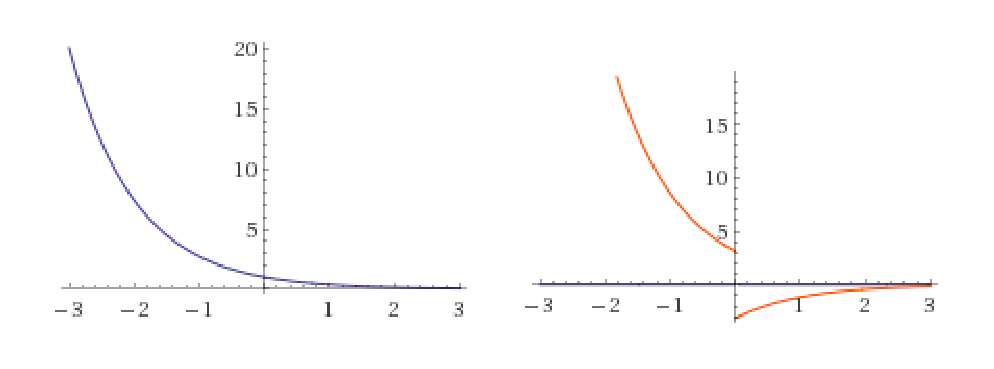
\includegraphics[width=\columnwidth]{fig/exp.pdf}
\caption{\label{fig:exp}Prubeh $e^{-rp}$ vlevo, prubeh $-\pi j \operatorname{sign}(p) e^{-r|p|}$ vpravo}
\end{figure}

\newpage

\subsection{b) Vypoctete Fourierovu transformaci funkce $f(t)\operatorname{sin}(2t)$}

Jako prvni krok si nahradime funkce $sin(2t)$ a to:
$$g(t)=f(t)\frac{e^{2t}-e^{-2t}}{2j}$$
Opet pokud tento vzorec jeste nikde nemate, doporucuji si ho napsat. Pozor zde na konkretni dvojnasobny argument. Funkci $g(t)$ muzeme roztrhnout na dve samostatne casti:
$$g(t) = \frac{1}{2j}f(t)e^{2t}-\frac{1}{2j}f(t)e^{-2t}$$
V clenech $e^{neco}$ opet pozorujeme vzorec, konkretne posun obrazu (\ref{eq:p_obrazu}). Tedy Fourerova transformace je:
$$\hat{g}(p)=\frac{1}{2j}\hat{f}(p-2)-\frac{1}{2j}\hat{f}(p+2)$$
Mohli byhom za funkci $\hat{f}(p)$ dosadit drive vypoctenou a vlastne vsechny promene $p$ nahradit bud $p-2$, ci $p+2$, ale zde to dle oficialnich vysledku stacilo vyjadrit obecne.

\newpage

\subsection{c) Vypoctete inverzni Fourierovu transformaci funkce $f(t)$}

Obcas muze byt matouci, ze mame inverzni Fourierovu transformaci, ktera prevede obraz $\hat{f}(p)$ zpet do casove oblasti, viz rovnice (\ref{eq:invF}). Ale take se nam objevuje definice inverzni Fourierovy transformace, ktera prevede $f(t)$ na $\check{f}(p)$ dle rovnice (\ref{eq:inv_ttop}), coz je presne tento nas konkretni pripad. Zde vyuzijeme toho, ze jsme si uz v bode a) spocetli primou Fourierovu transformaci a rovnice (\ref{eq:pain}), ktera rika, ze:
$$\hat{f}(p) = 2\pi \check{f}(-p)$$
My hledame $\check{f}(p)$, tedy to upravime:
$$\check{f}(-p) = \frac{1}{2\pi}\hat{f}(p)$$
A vyporadame se se znamenkem u $p$ prostym prohozenim:
$$\check{f}(p) = \frac{1}{2\pi}\hat{f}(-p)$$
Po dosazeni funkce $\hat{f}(p)$ tedy ziskame:
$$\check{f}(p) = \frac{1}{2\pi} \left(-\pi j \operatorname{sign}(-p) e^{-r|-p|} \right)$$
Vytkeneme znamkenko minus z funkce sign, coz se vynasobi se znamenkem minus pred celym zlomkem. Absolutni hodnota z $|-p|$ je to same jako $|p|$, takze to take muzeme zjednodusit.
$$\check{f}(p)=\frac{1}{2\pi} j \pi \operatorname{sign}(p) e^{-r|p|}$$
Mohli bychom treba jeste pokratit $\pi$, ale oficialni vysledek je tento. 

\textit{pozn: Uplne si nejsem jista, zda je korektni postup pouze prohodit znamenka misto $\check{f}(-p)$ a $\hat{f}(p)$. Kdyby to nekdo rozsiril o trochu teorie ci upravil, tak by to bylo fajn.}

\newpage

\section{a) Pomoci reziduove vety spoctete $\int_{-\infty}^\infty \frac{1}{(t^2+1)(t^2+2)}e^{-jpt}dt$}

Tady nam vlastne v zadani uz poradili jak to mame resit. Jinak by take zadani klidne mohlo znit: Urcete Fourieruv obraz pro funkci $f(t)=\frac{1}{(t^2+1)(t^2+2)}$. Cely integral si tedy oznacim jako $\hat{f}(p) = \int_{-\infty}^\infty \frac{1}{(t^2+1)(t^2+2)}e^{-jpt}dt $ Dulezite je opet si uvedomit, ze se jedna o zlomek dvou polynomu, coz se resi prave aplikaci reziduove vety. Musime v prvni rade urcit koreny:

$$t=\pm j$$
$$t=\pm j\sqrt{2}$$
Tedy musime opet pouzit vzorec (\ref{eq:rac_imag}):
$$R(z)=\frac{1}{(\left( -\frac{z}{p}\right)^2+1)(\left( -\frac{z}{p}\right)^2+2)}=\frac{1}{\left(\frac{z^2}{p^2}+1\right) \left( \frac{z^2}{p^2}+2\right)}$$
Coz dale upravime:
$$R(z)=\frac{1}{\frac{z^2+p^2}{p^2}\cdot \frac{z^2+2p^2}{p^2}}=\frac{p^4}{(z^2+p^2)(z^2+2p^2)}=\frac{p^4}{(z-jp)(z+jp)(z-\sqrt{2}jp)(z+\sqrt{2}jp)}$$
A koreny toho zlomku jsou:
$$z=\pm jp$$
$$z = \pm \sqrt{2}jp$$
Jako vzdy nas zajimaji pouze ty lezici v kladne polorovine, musime pouzit fintu s absolutni hodnotou pro $p$, tedy vysledna rezidua, ktera bereme v uvahu jsou:
$$z=j|p| ; \; \; z=\sqrt{2}j|p|$$
Obe jsou s nasobnosti jedna. Urcime vysledek tedy pro kazdou zvlast a udelame jejich sumu, jak rika vzorec (\ref{eq:rez}):
$$\hat{f}(p)=\frac{2\pi j}{|p|}\left( \lim_{z \to j|p|} \frac{|p|^4}{(z+j|p|)(z^2+2|p|^2)}\cdot e^{jz} + \lim_{z \to \sqrt{2}j|p|} \frac{|p|^4}{(z^2+|p|^2)(z+\sqrt{2}j|p|)}\cdot e^{jz} \right)$$
Vypocteme limity:
$$\hat{f}(p)=\frac{2\pi j}{|p|}\left( \frac{|p|^4}{2j|p|\cdot (-|p|^2+2|p|^2)}\cdot e^{-|p|}+\frac{|p|^4}{(-2|p|^2+|p|^2)\cdot 2\sqrt{2}j|p|}\cdot e^{-\sqrt{2}|p|}\right)$$
V predchozich rovnicich se hojne vyuzilo vlastnosti:
$$j^2 = -1$$
Jeste dale upravime:
$$\hat{f}(p)=\frac{2\pi j}{|p|}\left( \frac{|p|^4}{2j|p|\cdot |p|^2}\cdot e^{-|p|}+\frac{|p|^4}{-|p|^2\cdot 2\sqrt{2}j|p|}\cdot e^{-\sqrt{2}|p|}\right)=\frac{2\pi j}{|p|}\left( \frac{|p|^2}{2j|p|}\cdot e^{-|p|}+\frac{|p|^2}{-2\sqrt{2}j|p|}\cdot e^{-\sqrt{2}|p|}\right)$$
Vytkneme co se da a take namisto $|p|^2$ muzeme psat pouze $p^2$, protoze u sudych mocnin nam absolutni hodnota nic nezmeni.
$$\hat{f}(p)=\frac{2\pi j p^2}{|p|2j|p|} \left( \frac{e^{-|p|}}{1} - \frac{e^{-\sqrt{2}|p|}}{\sqrt{2}}\right)=\pi \left(e^{-|p|} -  \frac{e^{-\sqrt{2}|p|}}{\sqrt{2}}\right)$$
Coz je oficialni vysledek, ale kdybychom to chteli jeste vysperkovat, mohli bychom usmernit zlomek s odmocninou ve jmenovateli, tedy:
$$\hat{f}(p) = \pi \left(e^{-|p|} -  \frac{\sqrt{2} e^{-\sqrt{2}|p|}}{2}\right)$$

\newpage

\subsection{b) Pomoci tohoto vysledku urcete Fourieruv obraz funkce $h(t)=\frac{1}{(4t^2+1)(4t^2+2)}$}
\textit{pozn.: v zadani je funkce oznacena $f(t)$, ja jsem si to zde prejmenovala na $h(t)$, aby to nematlo s oznacenim funke $f(t)$ z bodu a}

V tomto prikladu muzeme pozorovat, ze puvodni jmenovatel $(t^2+1)(t^2+2)$ se ve vysledku $\hat{f}(p)$ projevuje dvema cleny. My si tedy zadani $h(t)$ upravime, abychom se priblizili puvodnimu zadani, tedy:
$$h(t)=\frac{1}{((2t)^2+1)((2t)^2+2)}$$
Z toho vidime, ze nas to navadi na pouziti vzorce zmena meritka (\ref{eq:zm_meritka}). Tedy:
$$\hat{h}(p)=\frac{1}{|2|}\hat{f}\left( \frac{p}{2}\right)= \frac{\pi}{|2|} \left( e^{-\left( \frac{|p|}{|2|}\right)} -  \frac{e^{-\sqrt{2}\left( \frac{|p|}{|2|}\right)}}{\sqrt{2}} \right)$$
Kde muzeme jeste odstanit absolutni hodnoty u $|2|$, protoze to nic nezmeni:
$$\hat{h}(p)=\frac{\pi}{2} \left( e^{-\left( \frac{|p|}{2}\right)} -  \frac{e^{-\sqrt{2}\left( \frac{|p|}{2}\right)}}{\sqrt{2}} \right)$$
\textit{pozn.: Kdyby zmena meritka nebyla u obou stejna, zlomek $\frac{1}{|2|}$ by nebyl pred zavorkou, ale u kazdeho clenu v zavorce zvlast na zaklade konstanty pro zmenu meritka}

\newpage

\subsection{c) Pomoci tohoto vysledku urcete Fourieruv obraz funkce $g(t)= \frac{d}{dt}\frac{1}{(t^2+1)(t^2+2)}$}

Tedy zadani rika: $g(t) = f'(t)$. Toto nas vede na vzorec obraz derivace (\ref{eq:obr_derivace}), tedy:
$$\hat{g}(p) = jp\hat{f}(p)=jp \pi \left(e^{-|p|} -  \frac{e^{-\sqrt{2}|p|}}{\sqrt{2}}\right)$$
A mame hotovo, to byla rychlovka, co? :)

\newpage

\section{Naleznete funkci $f(t)$, pro kterou plati $f(t)*e^{-at^2}=e^{-bt^2}$, $a>b>0$}

Toto je priklad na konvoluci. Vyuzijeme vlastnoti Fourierovy transformace, ktera konvoluci prevede na nasobeni obrazu funkci. Tedy naleznene obraz $\hat{f}(p)$ funkce $f(t)$ a inverzni transformaci ho privede do casove oblasti a ziskame hledanou $f(t)$. Postupujeme nasledovne, potrebujeme si urci obraz funkce $g(t) = e^{-at^2}$, ktery mame ve vzorcich (\ref{eq:aena2}), tedy:

$$\hat{g}(p)= \frac{\sqrt{\pi}}{\sqrt{a}}e^{-\frac{p^2}{4a}}$$
Obdobne funkce $h(t) = e^{-bt^2}$:
$$\hat{h}(p)= \frac{\sqrt{\pi}}{\sqrt{b}}e^{-\frac{p^2}{4b}}$$
Rovnice ze zadani je tedy ve Fourierove transformaci:
$$\hat{f}(p)\cdot \hat{g}(p) = \hat{h}(p)$$
$$\hat{f}(p) \cdot \frac{\sqrt{\pi}}{\sqrt{a}}e^{-\frac{p^2}{4a}} = \frac{\sqrt{\pi}}{\sqrt{b}}e^{-\frac{p^2}{4b}}$$
Z ceho vytkenem tedy hledanou $\hat{f}(p)$:
$$\hat{f}(p) = \frac{\frac{\sqrt{\pi}}{\sqrt{b}}e^{-\frac{p^2}{4b}}}{\frac{\sqrt{\pi}}{\sqrt{a}}e^{-\frac{p^2}{4a}}}= \frac{\sqrt{a}}{\sqrt{b}}e^{-\frac{p^2}{4b}+\frac{p^2}{4a}}$$
Exponent chceme dostat pouze na jeden zlomek, tedy upravujeme:
$$\hat{f}(p)=\frac{\sqrt{a}}{\sqrt{b}}e^{-\frac{p^2}{4}\left( \frac{1}{b}-\frac{1}{a}\right)} =\frac{\sqrt{a}}{\sqrt{b}}e^{-\frac{p^2}{4} \frac{a-b}{ab}}$$

Funkci $f(t)$ ziskame z $\hat{f}(p)$ opet s vyuzitim funkce:
$$e^{-xt^2} \to \frac{\sqrt{\pi}}{\sqrt{x}}e^{-\frac{p^2}{4x}}$$
K tomu musime udelat dve upravy. Za prve upravit exponent:
$$\hat{f}(p)=\frac{\sqrt{a}}{\sqrt{b}}e^{-\frac{p^2}{4\frac{ab}{a-b}} }$$
Za druhe jeste potrebujeme upravit konstantu $\frac{\sqrt{a}}{\sqrt{b}}$ tak, aby nejak odpovidala $\frac{\sqrt{\pi}}{\sqrt{x}}$. Zde si musime uvedomit, jaky vliv ma konstanta ve Fourierove transformaci, tedy pouzita funkce muze byt i v tomto tvaru:
$$c\cdot e^{-xt^2} \to c\cdot \frac{\sqrt{\pi}}{\sqrt{x}}e^{-\frac{p^2}{4x}}$$
Z teto uvahy i vyjdeme. Chceme, aby konstanta pred nasi exponencialou mela tvar:
$$c\cdot \frac{\sqrt{\pi}}{\sqrt{\frac{ab}{a-b}}}$$
coz lze jeste upravit rozsekanim odmocnin na mensi casti (muzeme pouze u deleni a nasobeni! Ne u scitani/odecitani!)
$$c\cdot \frac{\sqrt{\pi}}{\frac{\sqrt{a} \sqrt{b}}{\sqrt{a-b}}}$$

\textit{pozn.:Zde se vyborne hodi vlastnost $a>b>0$, abychom nemeli zaporne cislo v odmocnine}
Ale nase konstanta ma tvar:
$$\frac{\sqrt{a}}{\sqrt{b}}$$
Pokud pozadavek a skutecnost dame do rovnosti, muzeme urcit, jaka je konstanta $c$, ktera nam to ovlivnuje (zpusobuje, ze nektere cleny se jakoby zkratily). Resime tedy:
$$c\cdot \frac{\sqrt{\pi}}{\frac{\sqrt{a} \sqrt{b}}{\sqrt{a-b}}}=\frac{\sqrt{a}}{\sqrt{b}}$$
$$c = \frac{\sqrt{a}}{\sqrt{b}} \cdot \frac{\sqrt{a} \sqrt{b}}{\sqrt{a-b}}\cdot \frac{1}{\sqrt{\pi}}$$
Coz se zkrati na:
$$c = \frac{a}{\sqrt{\pi}\sqrt{a-b}}$$

Takze muzeme napsat vysledek a to tedy:
$$f(t) =c\cdot e^{-\frac{ab}{a-b} t^2} = \frac{a}{\sqrt{\pi}\sqrt{a-b}} \cdot e^{-\frac{ab}{a-b} t^2} $$

\newpage

\section{Reste pomoci F-transformace diferencialni rovnici}
$$-\frac{d^2u(x)}{dx^2}+a^2u(x)=f(x)$$
$$-\infty<x<\infty; \; a>0$$

Diferencialni rovnici si za pomoci vzorce pro obraz derivace (\ref{eq:obr_derivace})prevedu:
$$-(jp)^2\hat{u}(p)+a^2 \hat{u}(p) = \hat{f}(p)$$
Upravim:
$$p^2\hat{u}(p)+a^2 \hat{u}(p) = \hat{f}(p)$$
Vytknu $\hat{u}(p)$, protoze to hledam:
$$\hat{u}(p)(p^2+a^2)=\hat{f}(p)$$
Vytknu jen $\hat{u}(p)$:
$$\hat{u}(p)=\frac{\hat{f}(p)}{p^2+a^2}$$
Potrebovali bychom urcit zpetnou Fourierovu transformaci pro funkci:
$$\hat{g}(p)=\frac{1}{p^2+a^2}$$
Pro takove prilezitosti je dobry mit par zakladnich funkci vypsanych, tato funkce nam pripomina:
$$e^{-a|t|} \to \frac{2a}{p^2+a^2}$$
viz rovnice (\ref{eq:enaabs}) nebo take prvni priklad ze zadani.
Rozsirim tedy nasi rovnici zlomkem $\frac{2a}{2a}$ (tedy jednickou, nic nemenim), abych danou funkci tam ziskala:
$$\hat{u}(p)=\frac{\hat{f}(p)}{p^2+a^2}\cdot \frac{2a}{2a} = \hat{f}(p) \cdot \frac{2a}{p^2+a^2} \cdot \frac{1}{2a}$$
Zlomek $\frac{1}{2a}$ je pouze konstanta. Nasobeni mezi obrazy dvou funkci nas vede na konvoluci danych funkci, tedy jiz v casove oblasti:
$$u(x) = \frac{1}{2a}\cdot f(x)*e^{-a|t|}$$
Coz lze jeste prepsat na integral s vyuzitim rovnice (\ref{eq:konvoluce}):
$$u(x) = \frac{1}{2a} \int_{-\infty}^\infty f(s)\cdot e^{-a|x-s|}ds$$




